\chapter{Fundamentação Teórica}

Este capítulo apresenta uma breve introdução sobre os conceitos tocados neste
trabalho. Primeiro, é abordado as partes do \textit{pipeline} de um compilador
de maneira a entender, ao menos superficialmente, os algoritmos usados.
Em seguida, discute-se conceitos de computação paralela e possíveis abordagens
de paralelismo.

\begin{section}{Compiladores}

\begin{subsection}{\textit{Analisadores léxicos e sintáticos}}

O primeiro passo na compilação é a análise léxica e sintática para a criação
da árvore abstrata. Estas duas peças se comunicam constantemente, conforme
ilustrado na Figura \ref{fig:lexico_sintatico}.

\begin{figure}
\tikzstyle{block} = [rectangle, draw, fill=white,
    text width=6em, text centered, rounded corners, node distance=9cm, auto, minimum height=2em]
\tikzstyle{line} = [draw, -latex]
\tikzstyle{cloud} = [draw, ellipse,fill=white, node distance=2cm,
    minimum height=2em]

\begin{center}
\scalebox{0.8}{
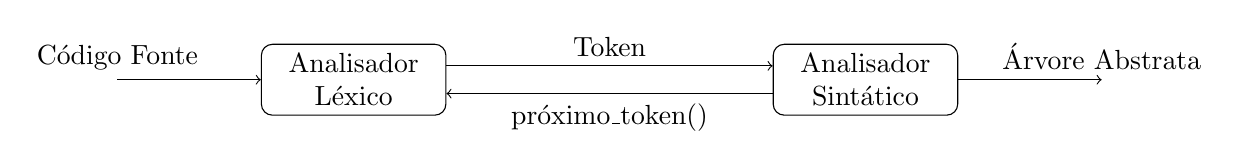
\begin{tikzpicture}[node distance = 3cm, auto]
    % Place nodes
    \node [block]                    (lexico) {Analisador Léxico};
    \node [block, right of = lexico] (sintatico) {Analisador Sintático};
    \coordinate [left of=lexico]     (fonte);
    \coordinate [right of=sintatico] (ast);

    % Draw edges
    \draw[->]    ([yshift=0.5em] lexico.east)       -- ([yshift=0.5em] sintatico.west) node[midway] {Token};
    \draw[->]    ([yshift=-0.5em] sintatico.west)   -- ([yshift=-0.5em] lexico.east)    node[midway] {próximo\_token()};
    \draw[->]    (fonte.west)                       -- (lexico.west)    node[pos=0, above] {Código Fonte};
    \draw[->]    (sintatico.east)                   -- (ast.west)   node[pos=1, above] {Árvore Abstrata};
\end{tikzpicture}
}
\end{center}

\caption{Interações entre um analisador léxico e sintático.}
\label{fig:lexico_sintatico}
\end{figure}

    Primeiro, a análise léxica é responsável por ler o arquivo
de texto contendo o código fonte, e quebrar as palavras em \textit{tokens}, que
serão alimentados para o analisador sintático. Por consequência, ele é capaz de
realizar alguns filtros como ignorar os comentários, identificar constantes
numéricas, eliminar espaços desnecessários,
entre outros. Analisadores léxicos também podem ser usados para substituição
de macros, como implementado pelo preprocessador do C
(CPP)\footnote{https://gcc.gnu.org/onlinedocs/cppinternals/Lexer.html}.

Geralmente, os analisadores léxicos são implementados utilizando autômatos por
serem $O(n)$, onde $n$ é o tamanho da entrada, pela existência de algoritmos
para converter expressões regulares em autômatos \citep{thompson}, e pela
existência de algoritmos para minimização de estados de um autômato
\citep{hopcroft1971n}. Isto possibilita que geradores de analisadores léxicos
como o \texttt{Flex}\footnote{https://www.gnu.org/software/flex/}
sejam bastante eficientes.

	Por fim, o analisador sintático entra em cena. O analisador sintático é
responsável por gerar a Árvore de Sintaxe Abstrata (AST) inspecionando a 
sequência de \textit{tokens} fornecido pelo analisador léxico. Neste processo,
ele certifica-se que o código fonte respeita a gramática da linguagem,
apontando erros caso contrário.

	Analisadores léxicos se apoiam nas gramáticas que geram uma
linguagem livre de contexto determinística, isto porque gramáticas mais
poderosas requerem algoritmos computacionalmente mais custosos
\citep{sipser2012}. Existem vários algoritmos para realizar a análise sintática,
mas destacam-se:
\begin{itemize}
    \item LL($k$): Um algoritmo de caráter preditivo, que tenta construir a AST da
        raiz para as folhas. Seu uso é devido a facilidade de codificação e
        mensagens de erros mais informativas para o usuário.

    \item LR($k$): Um algoritmo que tenta construir a AST das folhas para a raiz.
          Sua codificação é mais complicada e as mensagens de erro são mais
          precárias, porém são mais poderosos que o LL($k$) (toda gramática
          LL($k$) é LR($k$)). Outra vantagem interessante é a existência de
          \textit{softwares} como o
          \texttt{Bison}\footnote{https://www.gnu.org/software/bison/}, capaz
          de gerar um analisador LR($1$) a partir da especificação da gramática.
\end{itemize}

    Por fim, uma ação mais detalhada do funcionamento destes algoritmos
pode ser encontrada em \citep{appel2004modern}.

    Uma vez gerada a AST, é possível fazer verificações extras de semântica
relacionada a linguagem de programação, e em seguida essa AST normalmente é
traduzida para uma linguagem intermediária, onde serão feitas otimizações
no código.

Todo esse processo de analise léxica, sintática, e tradução
para a linguagem intermediária de uma linguagem é normalmente chamado de
\textit{frontend} de um compilador. Cada linguagem que o compilador aceita
como entrada contém um \textit{fronted} próprio, por exemplo, um para C,
outro para Fortran. Isto deixa o compilador mais modularizado, pois para
implementar uma nova linguagem de programação para o compilador, basta
implementar um novo \textit{frontend}.

\end{subsection}

\begin{subsection}{Linguagem Intermediária e Otimizações}

    Para um compilador ser capaz de compilar diversas linguagens como C, C++,
Fortran, normalmente é utilizado uma linguagem intermediária na qual a AST
será traduzida. Tal linugagem deve ser capaz de encapsular toda a
semântica da linguagem original, e permitir com que otimizações sejam
implementadas facilmente.

    Uma maneira de fazer isso é através de uma linugagem que represente
expressões em \textit{Three-Address code}. Aqui a expressão $a*x + b$ é
representado como

$$ t_1 = a*x$$
$$ t_2 = t_1 + b $$

    E para isso, novas variáveis são declaradas para conter os valores
intermediários possibilitando também a remoção de sub-expressões em comum.
Também neste modo, laços e o fluxo de código são transformados em
uma sequência de \texttt{if} e \texttt{goto} para facilitar a construção do
grafo de controle de fluxo. Com isto, é possível também eliminar código que
nunca será utilizado, e descartar variáveis que não são mais necessárias em
um certo ponto do programa. Todo esse processo normalmente é feito sem
analisar como as funções do programa interagem entre si.

    Para realizar otimizações considerando as interações entre as rotinas,
é utilizado um grafo de chamada de funções (\texttt{cgraphs}). Aqui as rotinas são
representadas como um vértice no grafo, e existe um arco de $f$ à $g$
quando há uma chamada de $g$ a partir de $f$. Dependendo da linguagem de
programação utilizada, construir tais grafos pode ser uma tarefa simples pois
as chamadas são normalmente feitas de modo estático, como é o caso de C; mas
isto pode se tornar algo extremamente complexo quando orientação à objetos é
empregada, pois é possível sobrescrever métodos.

    Os grafos de chamadas de funções permitem otimizações que eliminem chamadas
de funções, economizando assim o custo da chamada, e ainda permite com que as
funções sejam emitidas por ordem de proximidade, evitando com que o salto no
fluxo de execução seja demasiado longo, o que implicaria em \textit{cache miss}.
Também é possível descobrir que uma função não altera algum estado global, por exemplo,
imprimir na tela, e assim pré-computar o seu retorno em tempo de compilação. Por
exemplo:
    $$ \texttt{double pi = 4*atan(1.);}$$
Como a função \texttt{atan} não altera um estado global, \texttt{pi} poderia
ser computado em tempo de compilação. Grafos de chamada de funções também
permitem com que apenas funções que em tese serão chamadas sejam compiladas
apenas explorando a partir do ponto de entrada do programa, gerando assim
um binário menor.

    Após todo esse processo de otimização, o código em linguagem intermediária
pode ainda sofrer transformações em para algo que seja mais próximo do
\textit{hardware}-alvo, no caso da compilação ter como alvo código de máquina.
Um exemplo é o \textit{Register Transfer Language} (RTL) onde o código é
representado como uma sequência de instruções em uma máquina de infinitos
registradores. Finalmente, após essa sequência de transformações, o controle é
passado ao \textit{Backend} do compilador.

\end{subsection}

\begin{subsection}{Backend}
    É no \textit{Backend} do compilador que é implementado os assuntos
referentes à linguagem-alvo, como maneiras de imprimir rotinas, ou escolher
as instruções mais adequadas, expressando o código de uma maneira razoavelmente
eficiente. Esse tipo de modularização permite com que o compilador possa
suportar outra linguagem, ou outra máquina, apenas reimplementando o
\textit{Backend}.
\end{subsection}

\begin{figure}[ht]
\centering
  \begin{subfigure}[b]{0.40\textwidth}
	\tikzstyle{line} = [draw, -latex]
	\tikzstyle{node} = [draw, circle]
	\begin{center}
	\scalebox{0.8}{
	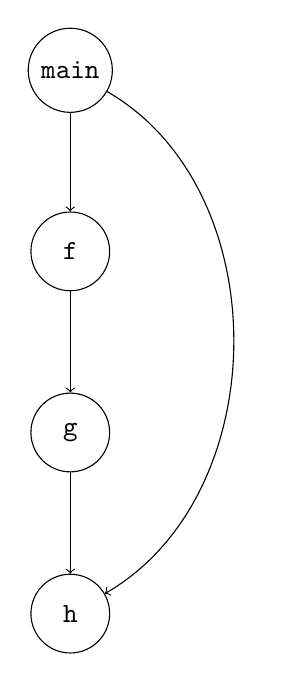
\begin{tikzpicture}[node distance = 2.3cm, minimum height = 1cm, auto]
		% Place nodes
		\node [node]                    (main) {\texttt{main}};
		\node [node, below of = main]    	 (f) {\texttt{f}};
		\node [node, below of = f]      	 (g) {\texttt{g}};
		\node [node, below of = g]      	 (h) {\texttt{h}};

		% Draw edges
		\draw[->]    (main)           -- (f);
		\draw[->]    (f)              -- (g);
		\draw[->]    (g)              -- (h);
		\draw[->]    (main)      to [out=-30,in=30] (h);
	\end{tikzpicture}
	}
	\end{center}
	\label{fig:call_graph}
  \end{subfigure}
  \begin{subfigure}[b]{0.40\textwidth}
	  \begin{lstlisting}[
		language=pseudocode,
		style=pseudocode,
		style=wider,
		functions={},
		specialidentifiers={extern, call},
	  ]
		extern function g,h

		function f()
			call $g$
			call $h$
		end

		function main()
			call $f$
			call $h$
		end
	  \end{lstlisting}
  \end{subfigure}
  \caption{Um programa e seu respectivo grafo de chamada de funções}
\end{figure}


\end{section}

\begin{section}{Computação Paralela}

\end{section}



\begin{section}{O compilador GCC}

\begin{subsection}{GNU Toolchain e as etapas da compilação}

\begin{figure}
\tikzstyle{block} = [rectangle, draw, fill=white,
    text width=6em, text centered, rounded corners, node distance=6.5cm, auto, minimum height=2em]
\tikzstyle{line} = [draw, -latex]
\tikzstyle{cloud} = [draw, ellipse,fill=white, node distance=2cm,
    minimum height=2em]
\begin{center}
\scalebox{0.7}{
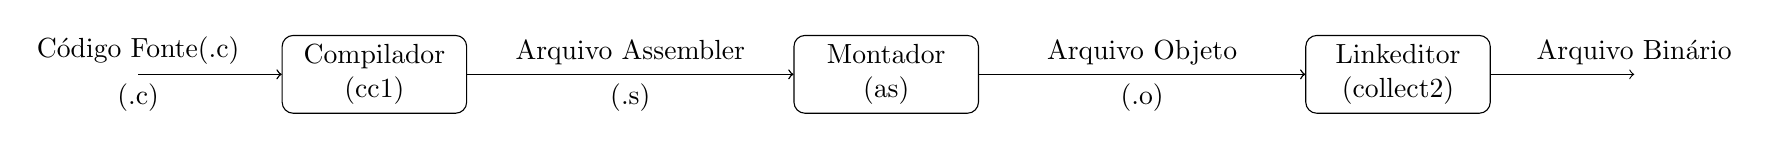
\begin{tikzpicture}[node distance = 3cm, auto]
    % Place nodes
    \node [block]                      (cc1) {Compilador \\ (cc1)};
    \node [block, right of = cc1]      (as) {Montador\\(as)};
    \node [block, right of = as]       (collect2) {Linkeditor\\(collect2)};
    \coordinate [left of=cc1]          (fonte);
    \coordinate [right of=collect2]    (bin);

    % Draw edges
    \draw[->]    (cc1.east)          -- (as.west)       node[midway, above] {Arquivo Assembler};
    \draw[->]    (cc1.east)          -- (as.west)       node[midway, below] {(.s)};
    \draw[->]    (as.east)           -- (collect2.west) node[midway, above] {Arquivo Objeto};
    \draw[->]    (as.east)           -- (collect2.west) node[midway, below] {(.o)};
    \draw[->]    (fonte.west)        -- (cc1.west)      node[pos=0, above] {Código Fonte\\ (.c)};
    \draw[->]    (fonte.west)        -- (cc1.west)      node[pos=0, below] {(.c)};
    \draw[->]    (collect2.east)     -- (bin.west)      node[pos=1, above] {Arquivo Binário};
\end{tikzpicture}
}
\end{center}

\caption{Etapas de Compilação.}
\label{fig:gnu_toolchain}
\end{figure}

\end{subsection}

\end{section}
